\section{Differentiating between Catch Categories}

As the basis for a simple length-based assessment tool for the data poor deep slope fisheries, we can now obtain values for all key length-based life history characteristics for all species in our target list. And by overlaying these values over accumulated catch length frequencies, we can ``split'' the catch of each species in major ``catch categories'', for example including:

\begin{enumerate}[noitemsep,topsep=0pt,parsep=0pt,partopsep=0pt]
\item \% in the catch < Lmat,
\item \% in the catch >= Lmat but < Lopt, and
\item \% in the catch >= Lopt.
\end{enumerate}

These ``catch categories'' are (1) the percentage of fish in the catch (in terms of numbers) that never reached maturity, (2) the percentage that reached maturity but never reached the optimum harvest size, and (3) the percentage of fish in the catch that has reached the optimal harvest size and lived to grow beyond that.

Looking at these percentages for an accumulated catch length frequency (over a year) will give us an indication of the current impact of the fishery by species. If mostly immature fish are included in the catch, for example, there is reason for concern and a closer look. Following the same percentages over time (from year to year) also enables us to look for signs of improvement (for example increasing percentage in category 2, while the percentage in category 1 decreases) or note signs of deterioration (increasing percentages in category 1 for example).

\section{Plotting Results from Length-Based Assessments}
Using key length-based life history characteristics for our target species, we are now able to apply a simple tool for the analysis of length frequency distributions in the landed catches, therewith stimulating a focused discussion among stakeholders on the impact and status of the fisheries. We can start with visualizing the accumulated catch (for example over 1 year) in terms of the lengths of the fish in relation to the values of the key life history characteristics. The position and shape of the length frequency distribution relative to the positions of these values gives us a first tool to start our length-based assessment. As a next step, we can plot the percentages from multiple years in each of the ``catch categories'' in a line graph to see how the situation develops over time. 

Figures 3 and 4 are examples of such plots with length frequency distributions of landings of \textit{Lutjanus fantasticus}, an imaginary species of snapper. Figure 3 shows a plot for a situation where a large percentage of the fish in the catch is still immature and was removed by the fishery before being able to spawn or reach their full growth potential. Figure 4 shows a situation where relatively more fish in the catch are already mature, have therefore spawned before being caught and are closer to the optimum length for harvesting that species. Figures 5 and 6 are examples of plots with percentages of the catch categories over multiple years. Figure 5 shows a situation where initially mostly juvenile snappers were caught, while in later years the catch shifts to more adult and larger animals. Figure 6 shows a situation where initially mostly large fish were caught but eventually only juveniles remain.

\begin{center}
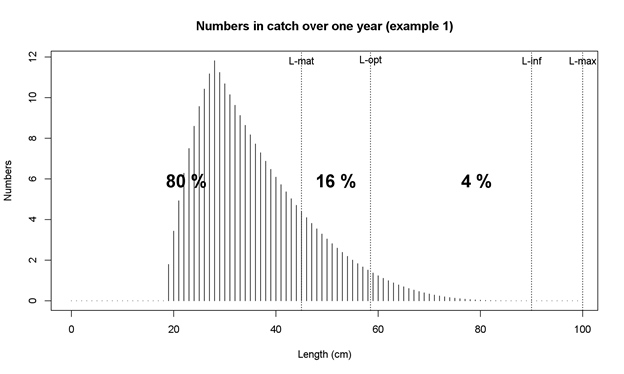
\includegraphics[width=.9\linewidth]{/root/R-project/IFishAssessmentGuide/Images/Figure-3.png}
\end{center}
\textbf{Figure 3.} Catch length frequency distribution of Lutjanus fantasticus for an example situation where a large percentage of the fish in the catch is still immature and was removed by the fishery before being able to spawn or reach the full growth potential. This is an example of a situation with overfishing including the targeting of juveniles.

\begin{center}
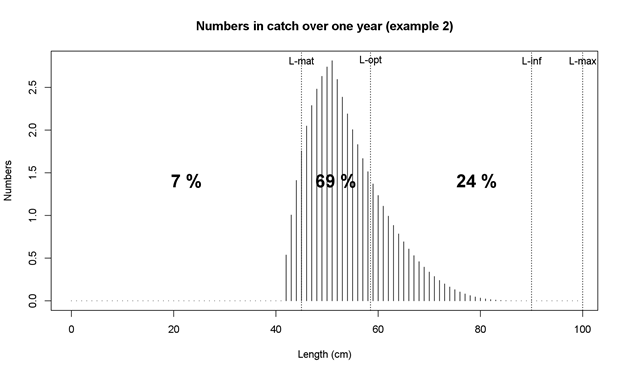
\includegraphics[width=.9\linewidth]{/root/R-project/IFishAssessmentGuide/Images/Figure-4.png}
\end{center}
\textbf{Figure 4.} Catch length frequency distribution of \textit{Lutjanus fantasticus} for an example situation where a large percentage of the fish in the catch is mature and was removed by the fishery after being able to spawn and approaching the full growth potential. This is an example of a more sustainable situation with the fisheries are mainly targeting adults.

\begin{center}
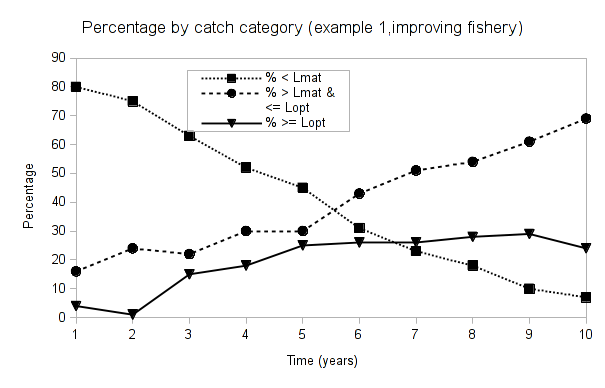
\includegraphics[width=.9\linewidth]{/root/R-project/IFishAssessmentGuide/Images/Figure-5.png}
\end{center}
\textbf{Figure 5.} Shift in catch categories of \textit{Lutjanus fantasticus} for an example situation where initially a large percentage of the fish in the catch is immature and was removed by the fishery before being able to spawn or reach full growth potential. Over the years, the situation improves with larger mature animals becoming more dominant in the catch.

\begin{center}
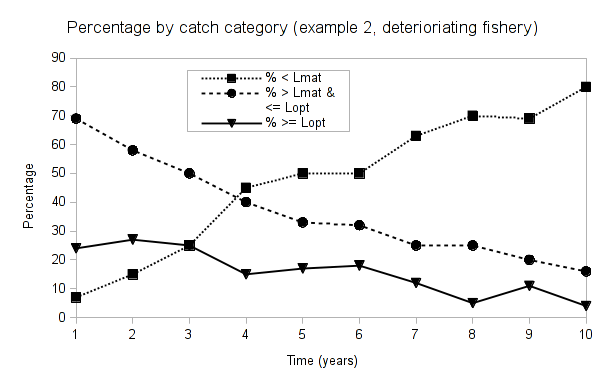
\includegraphics[width=.9\linewidth]{/root/R-project/IFishAssessmentGuide/Images/Figure-6.png}
\end{center}
\textbf{Figure 6.} Shift in catch categories of \textit{Lutjanus fantasticus} where initially a large percentage of the fish in the catch is mature and has approached their full growth potential. Over the years, the situation deteriorates with smaller immature animals becoming more dominant in the catch. This development would be a clear reason for concern.
